\documentclass[tikz,border=0pt]{standalone}
\pdfminorversion=7
\usepackage[T1]{fontenc}
\usepackage{lmodern,amsmath,amssymb,graphicx}
\usepackage{pgfplots}
\usetikzlibrary{arrows.meta,calc,positioning,patterns,decorations.pathreplacing}
\pgfplotsset{compat=1.18}
\definecolor{family}{RGB}{0,140,18}
\definecolor{familypale}{RGB}{225,255,226}
\definecolor{frozen}{RGB}{49,57,208}
\definecolor{frozenpale}{RGB}{234,235,255}
\definecolor{adapter}{RGB}{219,102,0}
\definecolor{adapterpale}{RGB}{255,196,135}
\definecolor{outputcol}{RGB}{120,38,130}
\definecolor{ink}{RGB}{33,33,33}
\definecolor{muted}{RGB}{105,105,105}
\tikzset{
 figure/.style={x=1pt,y=1pt,line cap=round,line join=round,text=ink,
   >={Stealth[length=7pt,width=6pt]},font=\fontsize{20}{24}\selectfont},
 title/.style={font=\fontsize{29}{33}\selectfont},
 heading/.style={font=\fontsize{22}{26}\selectfont},
 labeltext/.style={font=\fontsize{18}{22}\selectfont,align=center},
 smalllabel/.style={font=\fontsize{15}{19}\selectfont,align=center},
 equation/.style={font=\fontsize{24}{29}\selectfont,align=center},
 flow/.style={->,line width=1.3pt},
 fineflow/.style={->,line width=.8pt},
 target/.style={circle,fill=family,draw=white,line width=1.2pt,inner sep=0pt,minimum size=12pt},
 candidate/.style={circle,fill=white,draw=muted,line width=1.3pt,inner sep=0pt,minimum size=10pt},
 neuron/.style={circle,draw=frozen,fill=frozen!18,minimum size=13pt,inner sep=0pt,line width=.8pt}
}
\DeclareMathOperator{\rank}{rank}
\DeclareMathOperator{\row}{row}
\DeclareMathOperator{\col}{col}
\newcommand{\R}{\mathbb R}
\graphicspath{{assets/}}
\newcommand{\canvas}[1]{\path[use as bounding box] (0,0) rectangle (960,600);
  \node[title,anchor=west] at (36,557) {#1};}
\newcommand{\glyphgrid}[2]{
 \begin{scope}[shift={(#1,#2)}]
  \fill[white] (0,0) rectangle (136,136);
  \foreach \x/\y/\c in {1/1/80,2/2/80,2/3/45,3/4/45,3/5/45,4/5/100,4/6/45,5/6/45,5/4/45,5/2/100,6/1/80}{
    \fill[frozen!\c] (\x*17,\y*17) rectangle ++(17,17);
  }
  \draw[step=17pt,black!30,line width=.35pt] (0,0) grid (136,136);
  \draw[black!45,line width=.6pt] (0,0) rectangle (136,136);
 \end{scope}}

\begin{document}
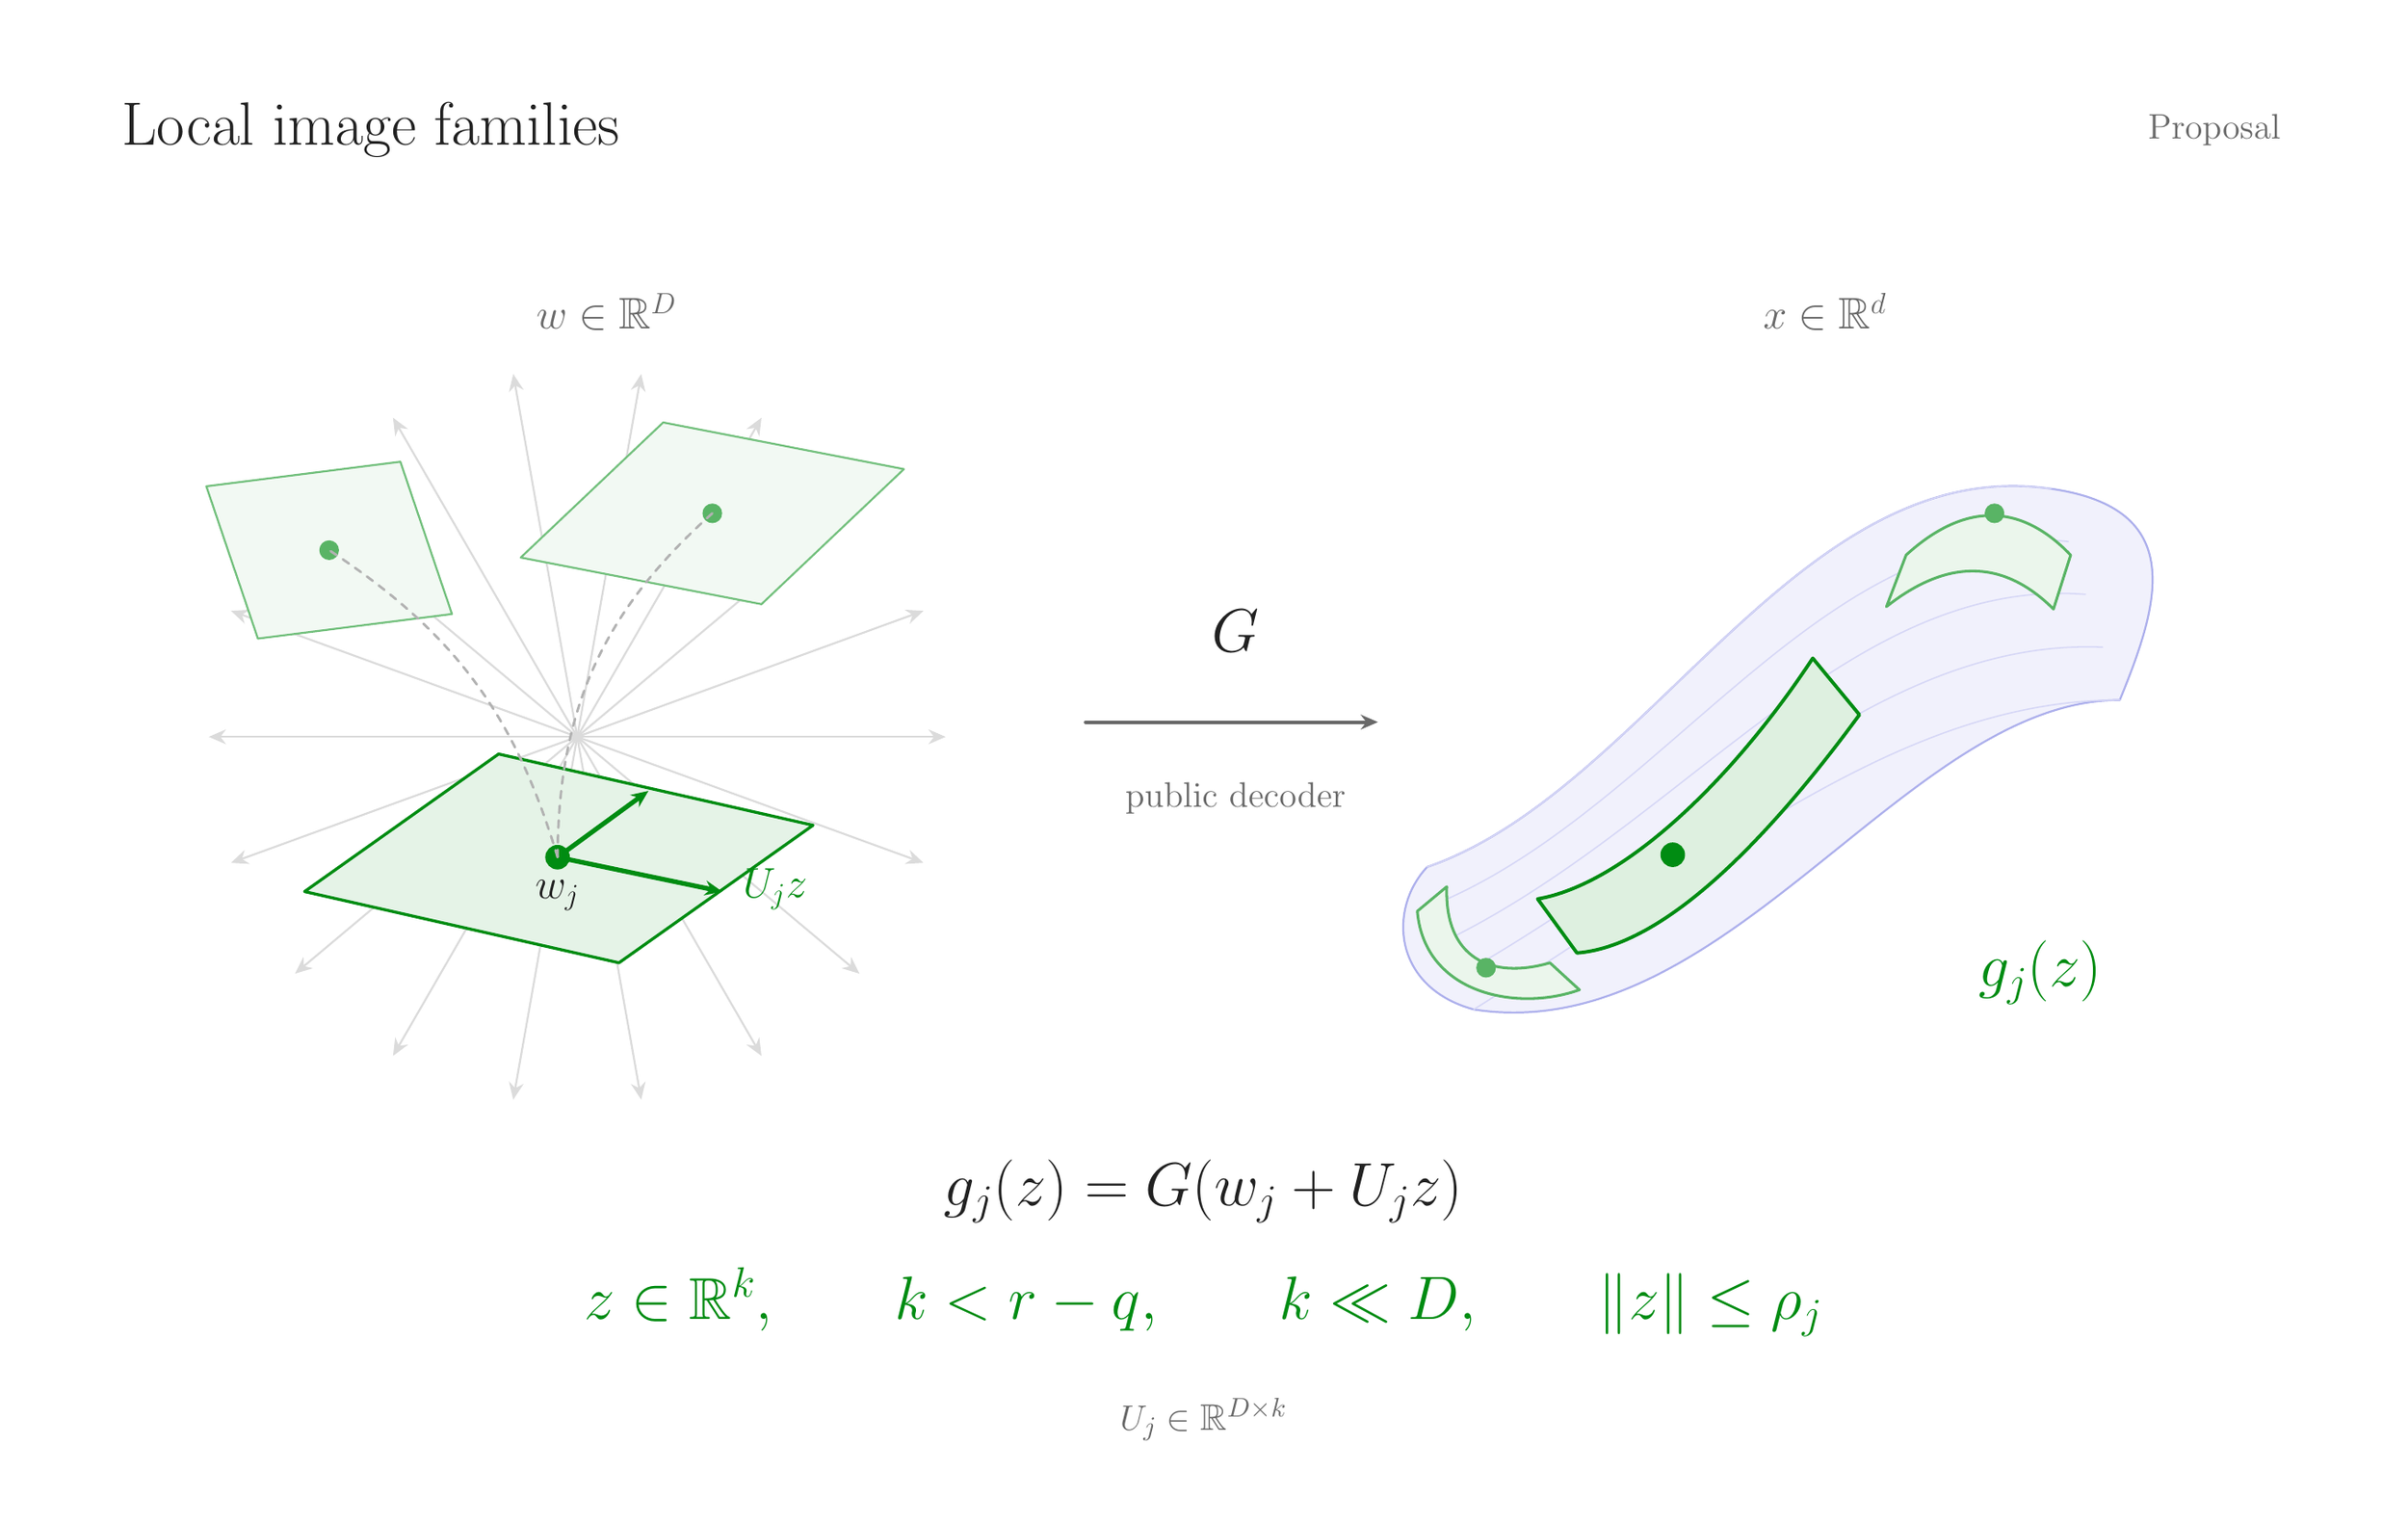
\begin{tikzpicture}[figure]
\canvas{Local image families}
\node[smalllabel,text=muted,anchor=east] at (922,557) {Proposal};
\node[labeltext,text=muted] at (237,483) {$w\in\R^D$};
\begin{scope}[shift={(225,310)}]
 \foreach \a in {0,20,40,60,80,100,120,140,160,180,200,220,240,260,280,300,320,340}
  \draw[black!14,fineflow] (0,0)--(\a:150);
 \filldraw[fill=family!10,draw=family,line width=1.2pt] (-111,-63)--(17,-92)--(96,-36)--(-32,-7)--cycle;
 \filldraw[fill=family!5,draw=family!55,line width=.8pt] (-23,73)--(75,54)--(133,109)--(35,128)--cycle;
 \filldraw[fill=family!5,draw=family!55,line width=.8pt] (-130,40)--(-51,50)--(-72,112)--(-151,102)--cycle;
 \fill[fill=family] (-8,-49) circle (5pt);
 \fill[family!65] (55,91) circle (4pt);
 \fill[family!65] (-101,76) circle (4pt);
 \draw[flow,draw=family,line width=1.9pt] (-8,-49)--(59,-63);
 \draw[flow,draw=family,line width=1.9pt] (-8,-49)--(29,-22);
 \node[labeltext,anchor=north] at (-8,-55) {$w_j$};
 \node[labeltext,text=family,anchor=west] at (64,-62) {$U_jz$};
 \draw[dashed,black!30,line width=1pt] (-8,-49) to[bend left=24] (55,91);
 \draw[dashed,black!30,line width=1pt] (-8,-49) to[bend right=20] (-101,76);
\end{scope}
\draw[flow,muted,line width=1.5pt] (432,316)--(551,316);
\node[equation] at (493,353) {$G$};
\node[smalllabel,text=muted] at (493,285) {public decoder};
\begin{scope}[shift={(727,302)}]
 \path[fill=frozen!7,draw=frozen!40,line width=.8pt]
  (-156,-45) .. controls (-66,-14) and (-5,124) .. (98,109)
  .. controls (154,101) and (142,62) .. (126,23)
  .. controls (39,23) and (-34,-119) .. (-137,-103)
  .. controls (-170,-94) and (-172,-62) .. (-156,-45);
 \foreach \t in {0,.25,.5,.75,1}{
  \draw[frozen!20,line width=.55pt]
   ({-156+19*\t},{-45-58*\t})
   .. controls ({-66+32*\t},{-14-24*\t}) and ({-5+44*\t},{124-101*\t}) ..
   ({98+28*\t},{109-86*\t});
 }
 \path[fill=family!13,draw=family,line width=1.4pt]
  (-111,-58) .. controls (-76,-52) and (-32,-10) .. (1,40)
  --(20,17) .. controls (-13,-28) and (-57,-77) .. (-95,-80)--cycle;
 \path[fill=family!8,draw=family!65,line width=1.1pt]
  (39,82) .. controls (62,103) and (85,104) .. (106,82)
  --(99,60) .. controls (78,81) and (55,80) .. (31,61)--cycle;
 \path[fill=family!8,draw=family!65,line width=1.1pt]
  (-148,-53) .. controls (-149,-82) and (-130,-91) .. (-106,-84)
  --(-94,-95) .. controls (-119,-104) and (-157,-97) .. (-160,-63)--cycle;
 \fill[fill=family] (-56,-40) circle (5pt);
 \fill[family!65] (75,99) circle (4pt);
 \fill[family!65] (-132,-86) circle (4pt);
 \node[equation,text=family,anchor=west] at (65,-88) {$g_j(z)$};
\end{scope}
\node[labeltext,text=muted] at (733,483) {$x\in\R^d$};
\node[equation] at (480,125) {$g_j(z)=G(w_j+U_jz)$};
\node[equation,text=family] at (480,80) {$z\in\R^k,\qquad k<r-q,\qquad k\ll D,\qquad\|z\|\le\rho_j$};
\node[smalllabel,text=muted] at (480,32) {$U_j\in\R^{D\times k}$};
\end{tikzpicture}
\end{document}
